\documentclass[8pt,a4paper,compress]{beamer}

\usepackage{/home/siyer/lib/slides}

\title{JVM Code Generation}
\date{}

\begin{document}
\begin{frame}
\vfill
\titlepage
\end{frame}

\section{Introduction}
\begin{frame}[fragile]
\pause

Once the AST has been fully analyzed, all variables and expressions have been typed, any necessary tree rewriting has been done, and a certain amount of setup needed for code generation has been accomplished

\pause
\bigskip

The compiler is now ready to traverse the AST one more time to generate the Java Virtual Machine (JVM) code, ie, build the class file for the program

\pause
\bigskip

For example, consider the following very simple program

\smallskip

\begin{lstlisting}[language=Java,style=focusin]
public class Square {
    public int square(int x) {
        return x * x;
    }
}
\end{lstlisting}

\pause
\bigskip

Compiling the program with our \jmm compiler

\smallskip

\begin{lstlisting}[language={},style=focusin]
$ $j/j--/bin/j-- Square.java
\end{lstlisting}
produces a class file \lstinline{Square.class}

\pause
\bigskip

Running the \lstinline{javap} program on the class file

\smallskip

\begin{lstlisting}[language={},style=focusin]
$ javap -verbose Square
\end{lstlisting}
produces the symbolic representation of the file shown in the next slide
\end{frame}

\begin{frame}[fragile]
\pause

\begin{lstlisting}[language={},style=focusin]
public class Square extends java.lang.Object
  minor version: 0
  major version: 49
  Constant pool:
const #1 = Asciz    Square;
const #2 = class    #1; //  Square
const #3 = Asciz    java/lang/Object;
const #4 = class    #3; //  java/lang/Object
const #5 = Asciz    <init>;
const #6 = Asciz    ()V;
const #7 = NameAndType  #5:#6;//  "<init>":()V
const #8 = Method   #4.#7;  //  java/lang/Object."<init>":()V
const #9 = Asciz    Code;
const #10 = Asciz   square;
const #11 = Asciz   (I)I;

{
public Square();
  Code:
   Stack=1, Locals=1, Args_size=1
   0: aload_0
   1: invokespecial #8; //Method java/lang/Object."<init>":()V
   4: return

public int square(int);
  Code:
   Stack=2, Locals=2, Args_size=2
   0: iload_1
   1: iload_1
   2: imul
   3: ireturn

}
\end{lstlisting}
\end{frame}

\begin{frame}[fragile]
\pause

To emit JVM instructions, we firstly create a \lstinline{CLEmitter} instance, which is an abstraction of the class file we wish to build, and then call upon \lstinline{CLEmitter}'s methods for generating the necessary headers and instructions

\pause
\bigskip

For example, to generate the class header

\smallskip

\begin{lstlisting}[language=Java,style=focusin]
public class Square extends java.lang.Object
\end{lstlisting}

\smallskip

we would invoke the \lstinline{addClass()} method on \lstinline{output}, an instance of \lstinline{CLEmitter}

\smallskip

\begin{lstlisting}[language=Java,style=focusin]
output.addClass(mods, "Square", "java/lang/Object", null, false);
\end{lstlisting}

\pause
\bigskip

As another example, the no-argument instruction \lstinline{aload_1} may be generated by

\smallskip

\begin{lstlisting}[language=Java,style=focusin]
output.addNoArgInstruction(ALOAD_1);
\end{lstlisting}
\end{frame}

\begin{frame}[fragile]
\pause

For a more involved example of code generation, consider the \lstinline{Factorial} program from before

\smallskip

\begin{lstlisting}[language=Java,style=focusin]
package pass;

import java.lang.System;

public class Factorial {
    // Two methods and a field

    public static int factorial(int n) {
        // position 1:
        if (n <= 0) {
            return 1;
        } else {
            return n * factorial(n - 1);
        }
    }

    public static void main(String[] args) {
        int x = n;

        // position 2:
        System.out.println(n + "! = " + factorial(x));
    }

    static int n = 5;
}
\end{lstlisting}
\end{frame}

\begin{frame}[fragile]
\pause

Running \lstinline{javap} on \lstinline{Factorial.class} produced by the \jmm compiler gives us

\smallskip

\begin{lstlisting}[language={},style=focusin]
public class pass.Factorial extends java.lang.Object
  minor version: 0
  major version: 49
  Constant pool:
  ...
{
static int n;

public pass.Factorial();
  Code:
   Stack=1, Locals=1, Args_size=1
   0: aload_0
   1: invokespecial #8; //Method java/lang/Object."<init>":()V
   4: return

public static int factorial(int);
  Code:
   Stack=3, Locals=1, Args_size=1
   0: iload_0
   1: iconst_0
   2: if_icmpgt 10
   5: iconst_1
   6: ireturn
   7: goto  19
   10: iload_0
   11: iload_0
   12: iconst_1
   13: isub
   14: invokestatic #13; //Method factorial:(I)I
   17: imul
   18: ireturn
   19: nop
\end{lstlisting}
\end{frame}

\begin{frame}[fragile]
\pause

\begin{lstlisting}[language={},style=focusin]


public static void main(java.lang.String[]);
  Code:
   Stack=3, Locals=2, Args_size=1
   0: getstatic #19; //Field n:I
   3: istore_1
   4: getstatic #25; //Field java/lang/System.out:Ljava/io/PrintStream;
   7: new   #27; //class java/lang/StringBuilder
   10: dup
   11: invokespecial    #28; //Method java/lang/StringBuilder."<init>":()V
   14: getstatic    #19; //Field n:I
   17: invokevirtual    #32; //Method java/lang/StringBuilder.append:
                             (I)Ljava/lang/StringBuilder;
   20: ldc  #34; //String ! =
   22: invokevirtual    #37; //Method java/lang/StringBuilder.append:
                             (Ljava/lang/String;)Ljava/lang/StringBuilder;
   25: iload_1
   26: invokestatic #13; //Method factorial:(I)I
   29: invokevirtual    #32; //Method java/lang/StringBuilder.append:
                             (I)Ljava/lang/StringBuilder;
   32: invokevirtual    #41; //Method java/lang/StringBuilder.toString:
                             ()Ljava/lang/String;
   35: invokevirtual    #47; //Method java/io/PrintStream.println:
                             (Ljava/lang/String;)V
   38: return

public static {};
  Code:
   Stack=2, Locals=0, Args_size=0
   0: iconst_5
   1: putstatic #19; //Field n:I
   4: return
}
\end{lstlisting}
\end{frame}

\section{Generating Code for Classes and their Members}
\begin{frame}[fragile]
\pause

\lstinline{JCompilationUnit.codegen()} drives the generation of code for classes; for each type (ie, class) declaration, it
\begin{itemize}
\pause
\item invokes \lstinline{codegen()} on the \lstinline{JClassDeclaration} for generating the code for that class,
\pause
\item writes out the class to a class file in the destination directory, and
\pause
\item adds the in-memory representation of the class to a list that stores such representations for all the classes within a compilation unit; this list is used in translating JVM byte code to native (SPIM) code
\end{itemize}

\begin{lstlisting}[language=Java,style=focusin]
public void codegen(CLEmitter output) {
    for (JAST typeDeclaration : typeDeclarations) {
         typeDeclaration.codegen(output);
         output.write();
         clFiles.add(output.clFile());
    }
}
\end{lstlisting}
\end{frame}

\begin{frame}[fragile]
\pause

\lstinline{JClassDeclaration.codegen()} does the following
\begin{itemize}
\pause
\item It computes the fully-qualified name for the class, taking any package name into account
\pause
\item It invokes an \lstinline{addClass()} on the \lstinline{CLEmitter} for adding the class header to the start of the class file
\pause
\item If there is no explicit constructor with no arguments defined for the class, it invokes the private method \lstinline{codegenImplicitConstructor()} to generate code for the implicit constructor as required by the language
\pause
\item It generates code for its members, by sending the \lstinline{codegen()} message to each of them.
\pause
\item If there are any static field initializations in the class declaration, then it invokes the private method \lstinline{codegenClassInit()} to generate the code necessary for defining a static block, a block of code that is executed after a class is loaded
\end{itemize}
\end{frame}

\begin{frame}[fragile]
\pause

\lstinline{JMethodDeclaration.codegen()}

\smallskip

\begin{lstlisting}[language=Java,style=focusin]
public void codegen(CLEmitter output) {
    output.addMethod(mods, name, descriptor, null, false);
    if (body != null) {
        body.codegen(output);
    }

    // Add implicit RETURN
    if (returnType == Type.VOID) {
        output.addNoArgInstruction(RETURN);
    }
}
\end{lstlisting}

\pause
\bigskip

\lstinline{JConstructorDeclaration.codegen()}

\smallskip

\begin{lstlisting}[language=Java,style=focusin]
public void codegen(CLEmitter output) {
    output.addMethod(mods, "<init>", descriptor, null, false);
    if (!invokesConstructor) {
        output.addNoArgInstruction(ALOAD_0);
        output.addMemberAccessInstruction(INVOKESPECIAL,
                ((JTypeDecl) context.classContext().definition())
                        .superType().jvmName(), "<init>", "()V");
    }
    // Field initializations
    for (JFieldDeclaration field : 
             definingClass.instanceFieldInitializations()) {
        field.codegenInitializations(output);
    }
    // And then the body
    body.codegen(output);
    output.addNoArgInstruction(RETURN);
}
\end{lstlisting}
\end{frame}

\begin{frame}[fragile]
\pause

Since the analysis phase has moved initializations, \lstinline{codegen()} for \lstinline{JFieldDeclaration} need only generate code for the field declaration itself

\pause
\bigskip

\lstinline{JFieldDeclaration.codegen()}

\smallskip

\begin{lstlisting}[language=Java,style=focusin]
public void codegen(CLEmitter output) {
    for (JVariableDeclarator decl : decls) {
	// Add field to class
        output.addField(mods, decl.name(), decl.type()
            .toDescriptor(), false);
    }
}
\end{lstlisting}
\end{frame}

\section{Generating Code for Control and Logical Expressions}
\begin{frame}[fragile]
\pause

Almost all control statements in \jmm are controlled by some Boolean expression

\pause
\bigskip

For example, consider the if-then-else statement below

\smallskip

\begin{lstlisting}[language=Java,style=focusin]
if (a > b) { c = a; } else { c = b; }
\end{lstlisting}

The JVM code produced for the statement is as follows

\smallskip

\begin{lstlisting}[language={},style=focusin]
0: iload_1
1: iload_2
2: if_icmple 10
5: iload_1
6: istore_3
7: goto  12
10: iload_2
11: istore_3
12: ...
\end{lstlisting}

\pause
\bigskip

Notice a couple of things
\begin{enumerate}
\pause
\item We don't compute a Boolean value onto the stack and then branch on its value, but make use of the underlying JVM instruction set, which makes for more compact code

\pause
\item We branch to the else-part if the condition is \lstinline{false}

\smallskip

\begin{lstlisting}[language={},style=focusin]
branch to elseLabel if <condition> is false
    <code for thenPart>
    branch to endLabel
elseLabel:
    <code for elsePart>
endLabel:
\end{lstlisting}
\end{enumerate}
\end{frame}

\begin{frame}[fragile]
\pause

Suppose we wish implement the Java do-while statement in \jmm; for example

\smallskip

\begin{lstlisting}[language=Java,style=focusin]
do {
    a++;
}
while (a < b);
\end{lstlisting}

The code we generate might have the form

\smallskip

\begin{lstlisting}[language={},style=focusin]
topLabel:
    <code for body>
    branch to topLabel if <condition> is true
\end{lstlisting}

Note that we branch when the condition is \lstinline{true}

\pause
\bigskip

In generating code for a condition, one needs a method specifying three arguments
\begin{enumerate}
\pause
\item The \lstinline{CLEmitter} instance

\pause
\item The target label for the branch

\pause
\item A \lstinline{boolean} flag \lstinline{onTrue}; if \lstinline{onTrue} is \lstinline{true} then the branch should be made on the condition, and if \lstinline{false}, the branch should be made on the condition's complement
\end{enumerate}

\pause
\bigskip

Thus, every boolean expression must support a version of \lstinline{codegen()} with these three arguments;  for example, here is that overloaded \lstinline{codegen()} method for \lstinline{JGreaterThanOp}

\smallskip

\begin{lstlisting}[language=Java,style=focusin]
public void codegen(CLEmitter output, String targetLabel, boolean onTrue) {
    lhs.codegen(output);
    rhs.codegen(output);
    output.addBranchInstruction(onTrue ? IF_ICMPGT : IF_ICMPLE, targetLabel);
}
\end{lstlisting}
\end{frame}

\begin{frame}[fragile]
\pause

The three-argument \lstinline{codegen()} method is invoked on the condition controlling execution

\pause
\bigskip

For example, the \lstinline{codegen()} method in \lstinline{JIfStatement} makes use of the three-argument \lstinline{codegen()} method in producing code for the if-then-else statement

\smallskip

\begin{lstlisting}[language=Java,style=focusin]
public void codegen(CLEmitter output) {
    String elseLabel = output.createLabel();
    String endLabel = output.createLabel();
    condition.codegen(output, elseLabel, false);
    thenPart.codegen(output);
    if (elsePart != null) {
        output.addBranchInstruction(GOTO, endLabel);
    }
    output.addLabel(elseLabel);
    if (elsePart != null) {
        elsePart.codegen(output);
        output.addLabel(endLabel);
    }
}
\end{lstlisting}
\end{frame}

\begin{frame}[fragile]
\pause

The semantics of Java, and so of \jmm, requires that the evaluation of expressions such as \lstinline{arg1 && arg2} be short-circuited, ie, if \lstinline{arg1} is \lstinline{false}, then \lstinline{arg2} is not evaluated

\pause
\bigskip

The code to be generated depends of whether the branch for the entire expression is to be made on \lstinline{true}, or on \lstinline{false}

\begin{lstlisting}[language={},style=focusin]
Branch to target when           Branch to target when
    arg1 && arg2 is true:                arg1 && arg2 is false:

    branch to skip if               branch to target if
        arg1 is false                    arg1 is false
    branch to target when           branch to target if
        arg2 is true                     arg2 is false
skip: ...
\end{lstlisting}
\end{frame}

\begin{frame}[fragile]
\pause

For example, the code generated for 

\smallskip

\begin{lstlisting}[language=Java,style=focusin]
if (a > b && b > c) { c = a; } else { c = b; }
\end{lstlisting}

would be

\begin{lstlisting}[language={},style=focusin]
0: iload_1
1: iload_2
2: if_icmple 15
5: iload_2
6: iload_3
7: if_icmple 15
10: iload_1
11: istore_3
12: goto 17
15: iload_2
16: istore_3
17: ...
\end{lstlisting}

\pause
\bigskip

The \lstinline{codegen()} method in \lstinline{JLogicalAndOp}

\smallskip

\begin{lstlisting}[language=Java,style=focusin]
public void codegen(CLEmitter output, String targetLabel, boolean onTrue) {
    if (onTrue) {
        String falseLabel = output.createLabel();
        lhs.codegen(output, falseLabel, false);
        rhs.codegen(output, targetLabel, true);
        output.addLabel(falseLabel);
    } else {
        lhs.codegen(output, targetLabel, false);
        rhs.codegen(output, targetLabel, false);
    }
}
\end{lstlisting}
\end{frame}

\begin{frame}[fragile]
\pause

Notice that our method prevents unnecessary branches to branches; for example, consider the slightly more complicated condition in

\smallskip

\begin{lstlisting}[language=Java,style=focusin]
if (a > b && b > c && c > 5) { c = a; } else { c = b; }

\end{lstlisting}

The JVM code produced for this targets the same exit on \lstinline{false}, for each of the \lstinline{&&} operations

\smallskip

\begin{lstlisting}[language={},style=focusin]
0:   iload_1
1:   iload_2
2:   if_icmple       18
5:   iload_2
6:   iload_3
7:   if_icmple       18
10:  iload_3
11:  iconst_5
12:  if_icmple       18
15:  iinc    1, -1
18:  ...
\end{lstlisting}

\pause
\bigskip

The \lstinline{codegen()} method in \lstinline{JLogicalNotOp}

\smallskip

\begin{lstlisting}[language=Java,style=focusin]
public void codegen(CLEmitter output, String targetLabel, boolean onTrue) {
    arg.codegen(output, targetLabel, !onTrue);
}
\end{lstlisting}
\end{frame}

\section{Generating Code for Message Expressions, Field Selection, and Array Expressions}
\begin{frame}[fragile]
\pause

The \lstinline{codegen()} method in \lstinline{JMessageExpression} proceeds as follows
\begin{enumerate}
\pause
\item If the message expression involves an instance message, \lstinline{codegen()} generates code for the target
\pause
\item The message invocation instruction is determined: \lstinline{invokevirtual} for instance messages and \lstinline{invokestatic} for static messages
\pause
\item The \lstinline{addMemberAccessInstruction()} method is invoked to generate the message invocation instruction; this method takes the following arguments
\begin{enumerate}[(a)]
\pause
\item The instruction (\lstinline{invokevirtual} or \lstinline{invokestatic})
\pause
\item The JVM name for the target's type
\pause
\item The message name
\pause
\item The descriptor of the invoked method, which was determined in analysis.
\end{enumerate}
\pause
\item If the message expression is being used as a statement expression and the return type of the method  is non-void, then the method \lstinline{addNoArgInstruction()} is invoked for generating a \lstinline{pop} instruction; this is necessary because executing the message expression will produce a result on top of the stack, and this result is to be thrown away
\end{enumerate}
\end{frame}

\begin{frame}[fragile]
\pause

For example, the code generated for 

\smallskip

\begin{lstlisting}[language=Java,style=focusin]
... = s.square(6);
\end{lstlisting}

\smallskip

would be

\smallskip

\begin{lstlisting}[language={},style=focusin]
aload s' # s' denotes offset of s
bipush  6
invokevirtual   #6; //Method square:(I)I
\end{lstlisting}

whereas the code generated for 

\smallskip

\begin{lstlisting}[language=Java,style=focusin]
s.square(6);
\end{lstlisting}

\smallskip

would be 

\smallskip

\begin{lstlisting}[language={},style=focusin]
aload s'
bipush  6
invokevirtual   #6; //Method square:(I)I
pop
\end{lstlisting}

\pause
\bigskip

We invoke static methods using the \lstinline{invokestatic} instruction; for example the following \jmm code

\smallskip

\begin{lstlisting}[language=Java,style=focusin]
... = Square.square(5);
\end{lstlisting}

\smallskip

where \lstinline{int square(int)} is a static method in \lstinline{Square}, would generate the following JVM code

\smallskip

\begin{lstlisting}[language={},style=focusin]
iconst_5
invokestatic    #5; //Method square:(I)I
\end{lstlisting}
\end{frame}

\begin{frame}[fragile]
\pause

The \lstinline{codegen()} method in \lstinline{JFieldSelection} works as follows
\begin{enumerate}
\pause
\item It generates code for its target; if the target is a class, no code is generated
\pause
\item The compiler must again treat the special case, \lstinline{a.length} where \lstinline{a} is an array; the code generated makes use of the special instruction, \lstinline{arraylength}
\pause
\item Otherwise, it is treated as a proper field selection; the field selection instruction is determined: \lstinline{getfield} for instance fields and \lstinline{getstatic} for static fields
\pause
\item The \lstinline{addMemberAccessInstruction()} method is invoked with the following arguments
\begin{enumerate}[(a)]
\pause
\item The instruction (\lstinline{getfield} or \lstinline{getstatic})
\pause
\item The JVM name for the target's type
\pause
\item The field name
\pause
\item The JVM descriptor for the type of the field, and so the type of the result
\end{enumerate}
\end{enumerate}
\end{frame}

\begin{frame}[fragile]
\pause

For example, the following code

\smallskip

\begin{lstlisting}[language=Java,style=focusin]
... = s.instanceField;
\end{lstlisting}

\smallskip

would be translated as

\smallskip

\begin{lstlisting}[language={},style=focusin]
aload s'
getfield instanceField
\end{lstlisting}

\smallskip

whereas the following code
\begin{lstlisting}[language=Java,style=focusin]
... = Square.staticField;
\end{lstlisting}

\smallskip

would be translated as

\smallskip

\begin{lstlisting}[language={},style=focusin]
getstatic staticField
\end{lstlisting}

\pause
\bigskip

Code generation for array access expressions is straightforward; for example, if the variable \lstinline{a} references an array object, and \lstinline{i} is an integer, then the following code

\smallskip

\begin{lstlisting}[language=Java,style=focusin]
... = a[i];
\end{lstlisting}

\smallskip

is translated to 

\smallskip

\begin{lstlisting}[language={},style=focusin]
aload a'
iload i'
iaload
\end{lstlisting}
\end{frame}

\section{Generating Code for Assignment and Similar Operations}
\begin{frame}[fragile]
\pause

Consider the simple assignment statement
\begin{lstlisting}[language=Java]
x = y;
\end{lstlisting}
which asks that the value of the variable \lstinline{y} be stored in variable \lstinline{x}

\pause
\bigskip

We want the $l$-value (address or location) for \lstinline{x} and the $r$-value (content or value) for \lstinline{y}

\pause
\bigskip

All expressions have $r$-values, but many have no $l$-values; for example, if \lstinline{a} is an array of ten integers, and \lstinline{o} is an object with field \lstinline{f}, \lstinline{C} is a class with static field \lstinline{sf}, and \lstinline{x} is a local variable, the following have both $l$-values and $r$-values 
\begin{lstlisting}[language={}]
a[3]
o.f
C.sf
x
\end{lstlisting}
while the following have $r$-values, but not $l$-values
\begin{lstlisting}[language={}]
5
x+5
Factorial.factorial(5)
\end{lstlisting}
\end{frame}

\begin{frame}[fragile]
\pause

The right-hand-side expression is compiled to produce code for computing its $r$-value and leaving it on the stack

\pause
\bigskip

For the left-hand-side, sometimes no code needs to be generated, as in the following example
\begin{lstlisting}[language=Java]
x = y;
\end{lstlisting}
produces
\begin{lstlisting}[language={}]
iload y'
istore x'
\end{lstlisting}

\pause
\bigskip

On the other hand, compiling
\begin{lstlisting}[language=Java]
a[x] = y;
\end{lstlisting}
produces
\begin{lstlisting}[language={}]
aload a'
iload x'
iload y'
iastore
\end{lstlisting}

\pause
\bigskip

An assignment may act as a statement, as shown below
\begin{lstlisting}[language=Java]
x = y;
\end{lstlisting}
or as an expression, as shown below
\begin{lstlisting}[language=Java]
z = x = y;
\end{lstlisting}
\end{frame}

\begin{frame}[fragile]
\pause

In the first case, no value is left on the stack

\pause
\bigskip

In the second case, \lstinline{x = y} must assign the value of \lstinline{y} to \lstinline{x} but also leave a value (the $r$-value for \lstinline{y}) on the stack so that it may be popped off and assigned to \lstinline{z}, ie, the code might look something like
\begin{lstlisting}[language={}]
iload y'
dup
istore x'
istore z'
\end{lstlisting}

\pause
\bigskip

In parsing, when an expression is used as a statement, \lstinline{Parser}'s \lstinline{statementExpression()} method sets a flag \lstinline{isStatementExpression} in the expression node to \lstinline{true}, and the code generation phase makes use of this flag in deciding when code must be produced for duplicating $r$-values on the run-time stack

\pause
\bigskip

The most important property of the assignment is its side effect; one uses the assignment operation for its side effect: overwriting a variable's $r$-value with another

\pause
\bigskip

There are several Java (and \jmm) operations having the same sort of side effect; for example,
\begin{lstlisting}[language=Java]
x--
++x
x += 6
\end{lstlisting}
\end{frame}

\begin{frame}[fragile]
\pause

The table below compares the various operations (labeled down the left), with an assortment of left-hand sides (labeled across the top)
\begin{center}
\visible<2->{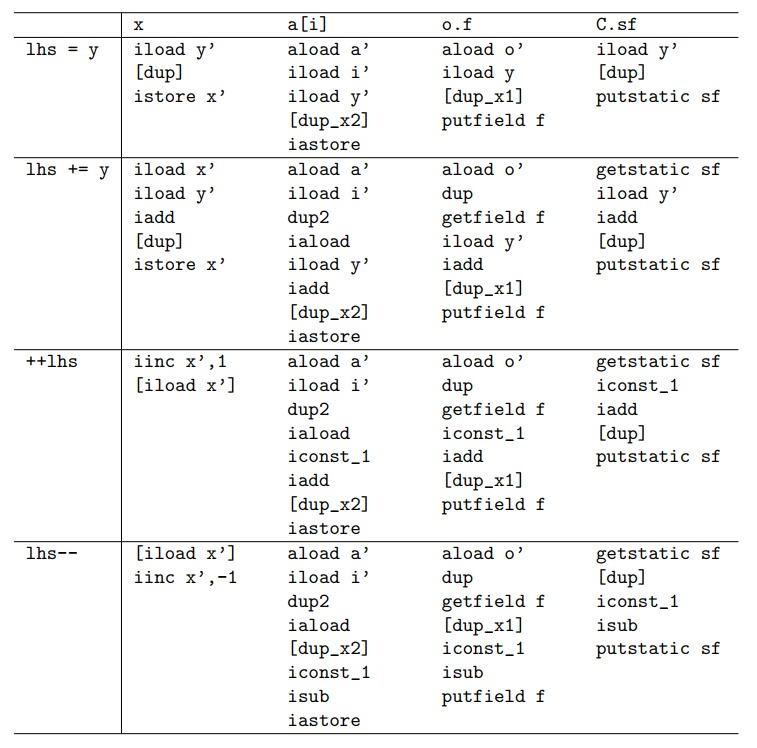
\includegraphics[scale=0.25]{{figures/assignments1}.jpg}}
\end{center}
The instructions in brackets [...] must be generated if and only if the operation is a sub-expression of some other expression, ie, if the operation is not a statement expression
\end{frame}

\begin{frame}[fragile]
\pause

The table above suggests four sub-operations common to most of the assignment-like operations in \jmm \begin{enumerate}
\pause
\item \lstinline{codegenLoadLhsLvalue()} - this generates code to load any up-front data for the left-hand side of an assignment needed for an eventual store, ie, its $l$-value
\pause
\item \lstinline{codegenLoadLhsRvalue()} - this generates code to load the $r$-value of the left-hand side, needed for implementing, for example the \lstinline{+=} operator
\pause
\item \lstinline{codegenDuplicateRvalue()} - this generates code to duplicate an $r$-value on the stack and put it in a place where it will be on top of the stack once the store is executed
\pause
\item \lstinline{codegenStore()} - this generates the code necessary to perform the actual store
\end{enumerate}

\pause
\bigskip

The code needed for each of these differs for each potential left-hand side of an assignment: a simple local variable \lstinline{x}, an indexed array element \lstinline{a[i]}, an instance field \lstinline{o.f}, and a static field \lstinline{C.sf}

\pause
\bigskip

The code necessary for each of the four operations, and for each left-hand-side form, is illustrated in the table below

\begin{center}
\visible<8->{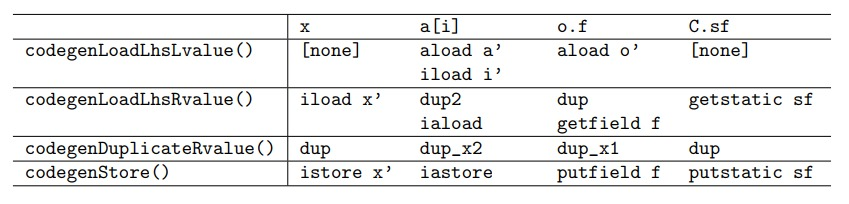
\includegraphics[scale=0.27]{{figures/assignments2}.jpg}}
\end{center}
\end{frame}

\begin{frame}[fragile]
\pause

Our compiler defines an interface \lstinline{JLhs}, which declares four abstract methods for these four sub-operations; each of \lstinline{JVariable}, \lstinline{JArrayExpression} and \lstinline{JFieldSelection} implements \lstinline{JLhs}

\pause
\bigskip

Of course, one must also be able to generate code for the right-hand side expression, but \lstinline{codegen()} is sufficient for that

\pause
\bigskip

For example, \lstinline{JPlusAssignOp}'s \lstinline{codegen()} is shown below
\begin{lstlisting}[language=Java,style=focusin]
public void codegen(CLEmitter output) {
    ((JLhs) lhs).codegenLoadLhsLvalue(output);
    if (lhs.type().equals(Type.STRING)) {
        rhs.codegen(output);
    } else {
        ((JLhs) lhs).codegenLoadLhsRvalue(output);
        rhs.codegen(output);
        output.addNoArgInstruction(IADD);
    }
    if (!isStatementExpression) {
        // Generate code to leave the r-value atop stack
        ((JLhs) lhs).codegenDuplicateRvalue(output);
    }
    ((JLhs) lhs).codegenStore(output);
}
\end{lstlisting}
\end{frame}

\section{Generating Code for String Concatenation}
\begin{frame}[fragile]
\pause

In \jmm, as in Java, the binary \lstinline{+} operator is overloaded; if both of its operands are integers, it denotes addition, but if either operand is a string then the operator denotes string concatenation and the result is a string

\pause
\bigskip

The compiler's analysis phase determines whether or not string concatenation is implied, and when it is, the concatenation is made explicit, ie, the operation's AST is rewritten, replacing \lstinline{JPlusOp} with a \lstinline{JStringConcatenationOp}

\pause
\bigskip

Also, when \lstinline{x} is a string, analysis replaces
\begin{lstlisting}[language=Java]
x += <expression>
\end{lstlisting}
by
\begin{lstlisting}[language=Java]
x = x + <expression>
\end{lstlisting}
\end{frame}

\begin{frame}[fragile]
\pause

To implement string concatenation, the compiler generates code to do the following
\begin{enumerate}
\pause
\item Create an empty string buffer, ie, a \lstinline{StringBuffer} object, and initialize it
\pause
\item Append any operands to that buffer; that \lstinline{StringBuffer}'s \lstinline{append()} method is overloaded to deal with any type makes handling operands of mixed types easy
\pause
\item Invoke the \lstinline{toString()} method on the string buffer to produce a \lstinline{String}
\end{enumerate}

\pause
\bigskip

\lstinline{JStringConcatenationOp}'s \lstinline{codegen()} makes use of a helper method, \lstinline{nestedCodegen()} for performing only step 2 for any nested string concatenation operations, which eliminates the instantiation of unnecessary string buffers

\pause
\bigskip

For example, given the \jmm expression
\begin{lstlisting}[language=Java,style=focusin]
x + true + "cat" + 0
\end{lstlisting}
the compiler generates the following JVM code
\begin{lstlisting}[language={},style=focusin]
new java/lang/StringBuilder
dup
invokespecial StringBuilder."<init>":()V
aload x'
invokevirtual append:(Ljava/lang/String;)StringBuilder;
iconst_1
invokevirtual append:(Z)Ljava/lang/StringBuilder;
ldc "cat"
invokevirtual append:(Ljava/lang/String;)Ljava/lang/StringBuilder;
iconst_0
invokevirtual append:(I)Ljava/lang/StringBuilder;
invokevirtual StringBuilder.toString:()Ljava/lang/String;
\end{lstlisting}
\end{frame}

\section{Generating Code for Casts}
\begin{frame}[fragile]
\pause

Analysis determines both the validity of a cast and the necessary \lstinline{Converter}, which encapsulates the code generated for the particular cast

\pause
\bigskip

Each \lstinline{Converter} implements a method \lstinline{codegen()}, which generates any code necessary to the cast

\pause
\bigskip

For example, consider the converter for casting a reference type to one of its sub-types (narrowing cast) which requires that a \lstinline{checkcast} instruction be generated
\begin{lstlisting}[language=Java,style=focusin]
class NarrowReference implements Converter {
    private Type target;

    public NarrowReference(Type target) {
        this.target = target;
    }

    public void codegen(CLEmitter output) {
        output.addReferenceInstruction(CHECKCAST, target.jvmName());
    }
}
\end{lstlisting}

\pause
\bigskip

On the other hand, when any type is cast to itself (the identity cast), or when a reference type is cast to one of its super types (called widening), no code need be generated
\end{frame}

\begin{frame}[fragile]
\pause

Casting an \lstinline{int} to an \lstinline{Integer} is called boxing and requires an invocation of the \lstinline{Integer.valueOf()} method

\begin{lstlisting}[language={},style=focusin]
invokestatic java/lang/Integer.valueOf:(I)Ljava/lang/Integer;
\end{lstlisting}

\pause
\bigskip

Casting an \lstinline{Integer} to an \lstinline{int} is called unboxing and requires an invocation of the \lstinline{Integer.intValue()} method

\begin{lstlisting}[language={},style=focusin]
invokevirtual java/lang/Integer.intValue:()I
\end{lstlisting}

\pause
\bigskip

Certain casts, from one primitive type to another require that a special instruction be executed; for example, the \lstinline{i2c} instruction converts an \lstinline{int} to a \lstinline{char}

\pause
\bigskip

There is a \lstinline{Converter} defined for each valid conversion in \jmm
\end{frame}
\end{document}
